% ═══════════════════════════════════════════════════════════════════════
% A1 Academic Poster — Solving 2048: Classical RL vs. LLM-Guided RLVR
% Full rewrite: poster-scale fonts, no whitespace, DoE + Findings
% ═══════════════════════════════════════════════════════════════════════
\documentclass[a1paper,portrait]{article}

% ── Geometry ──────────────────────────────────────────────────────────
\usepackage[a1paper, margin=0.85cm, top=0.6cm, bottom=0.6cm]{geometry}

% ── Packages ──────────────────────────────────────────────────────────
\usepackage{multicol}
\setlength{\columnsep}{1.0cm}
\setlength{\columnseprule}{0pt}
\usepackage{graphicx}
\usepackage{xcolor}
\usepackage{tikz}
\usetikzlibrary{shapes.geometric, arrows.meta, positioning, calc}
\usepackage{tcolorbox}
\tcbuselibrary{skins}
\usepackage{amsmath, amssymb}
\usepackage{booktabs}
\usepackage{enumitem}
\usepackage{array}
\usepackage{colortbl}
\usepackage[T1]{fontenc}
\usepackage{tgheros}
\renewcommand{\familydefault}{\sfdefault}

% ── Poster-scale font sizes (A1 requires ~18pt body for 1m readability)
\makeatletter
\renewcommand\normalsize{%
  \@setfontsize\normalsize{18}{23}%
  \abovedisplayskip 10\p@ \@plus2\p@ \@minus5\p@
  \belowdisplayskip\abovedisplayskip
  \abovedisplayshortskip \z@ \@plus3\p@
  \belowdisplayshortskip 6\p@ \@plus3\p@ \@minus3\p@
  \let\@listi\@listI}
\renewcommand\small      {\@setfontsize\small      {15}{19}}
\renewcommand\footnotesize{\@setfontsize\footnotesize{13}{17}}
\renewcommand\scriptsize {\@setfontsize\scriptsize {12}{15}}
\renewcommand\tiny       {\@setfontsize\tiny       {10}{13}}
\renewcommand\large      {\@setfontsize\large      {22}{27}}
\renewcommand\Large      {\@setfontsize\Large      {26}{32}}
\renewcommand\LARGE      {\@setfontsize\LARGE      {32}{38}}
\renewcommand\huge       {\@setfontsize\huge       {42}{50}}
\renewcommand\Huge       {\@setfontsize\Huge       {54}{64}}
\makeatother
\normalsize

\pagestyle{empty}
\setlength{\parindent}{0pt}
\setlength{\parskip}{0pt}

% ── Color palette ─────────────────────────────────────────────────────
\definecolor{headerbg}  {HTML}{8B0000}
\definecolor{accent}    {HTML}{C0392B}
\definecolor{sectioncolor}{HTML}{2C3E50}
\definecolor{dqncolor}  {HTML}{D35400}
\definecolor{dqnlight}  {HTML}{FEF9E7}
\definecolor{success}   {HTML}{1A7A4C}
\definecolor{successlight}{HTML}{EAF7F0}
\definecolor{danger}    {HTML}{C0392B}
\definecolor{dangerlight}{HTML}{FDEDEC}
\definecolor{info}      {HTML}{1F618D}
\definecolor{infolight} {HTML}{EBF5FB}
\definecolor{purple}    {HTML}{6C3483}
\definecolor{purplelight}{HTML}{F4ECF7}
\definecolor{darktext}  {HTML}{2C3E50}
\definecolor{codebg}    {HTML}{F2F3F4}
\definecolor{boardbg}   {HTML}{BBADA0}
\definecolor{emptycell} {HTML}{CDC1B4}
\definecolor{tile2}     {HTML}{EEE4DA}
\definecolor{tile4}     {HTML}{EDE0C8}
\definecolor{tile8}     {HTML}{F2B179}
\definecolor{tile32}    {HTML}{F67C5F}
\definecolor{tile64}    {HTML}{F65E3B}
\definecolor{tile128}   {HTML}{EDCF72}
\definecolor{tile256}   {HTML}{EDCC61}
\definecolor{tile512}   {HTML}{EDC850}
\definecolor{tile1024}  {HTML}{EDC53F}

% ── Box styles ────────────────────────────────────────────────────────
\newtcolorbox{sectionbox}[2][]{%
  enhanced, colback=white, colframe=#2, coltitle=white,
  fonttitle=\small\bfseries, title=#1,
  boxrule=2pt, arc=5pt,
  left=7pt, right=7pt, top=4pt, bottom=5pt,
  toptitle=4pt, bottomtitle=4pt,
  before skip=0pt, after skip=4pt,
  drop fuzzy shadow=black!12,
}

\newtcolorbox{calloutbox}[1][info]{%
  enhanced, colback=#1!8, colframe=#1!50,
  boxrule=0pt, arc=3pt,
  left=7pt, right=7pt, top=3pt, bottom=3pt,
  before skip=3pt, after skip=0pt,
  borderline west={3.5pt}{0pt}{#1},
}

\newtcolorbox{highlightbox}[1][accent]{%
  enhanced, colback=#1!8, colframe=#1,
  boxrule=2pt, arc=4pt,
  left=8pt, right=8pt, top=5pt, bottom=5pt,
  before skip=0pt, after skip=3pt,
}

\newtcolorbox{codebox}{%
  enhanced, colback=codebg, colframe=darktext!20,
  boxrule=0.5pt, arc=3pt,
  left=5pt, right=5pt, top=3pt, bottom=3pt,
  before skip=0pt, after skip=0pt,
}

% ── Helpers ───────────────────────────────────────────────────────────
\newcommand{\sectiontitle}[1]{%
  \vspace{1pt}{\color{sectioncolor}\Large\bfseries #1}\par
  {\color{accent}\rule{\linewidth}{2.5pt}}\par\vspace{1pt}}
\newcommand{\customtag} {{\tiny\colorbox{dqncolor} {\color{white}\bfseries\;Custom PyTorch\;}}}
\newcommand{\sbtag}     {{\tiny\colorbox{info}     {\color{white}\bfseries\;Stable-Baselines3\;}}}
\newcommand{\numpytag}  {{\tiny\colorbox{success}  {\color{white}\bfseries\;Custom NumPy\;}}}
\newcommand{\grpotag}   {{\tiny\colorbox{purple}   {\color{white}\bfseries\;trl + transformers\;}}}

% Transparent wrapper: ensures left-column text starts at same
% vertical position as the right-column codebox (both tcolorboxes
% start at 0pt, eliminating the [t]-minipage topskip offset).
\newtcolorbox{parambox}{%
  enhanced, colback=white, colframe=white,
  boxrule=0pt, arc=0pt, sharp corners,
  left=0pt, right=0pt, top=0pt, bottom=0pt,
  boxsep=0pt, before skip=0pt, after skip=0pt,
}

% ═══════════════════════════════════════════════════════════════════════
\begin{document}
\color{darktext}

% ── HEADER ────────────────────────────────────────────────────────────
\begin{tcolorbox}[
  enhanced, colback=headerbg, colframe=headerbg,
  boxrule=0pt, arc=0pt,
  left=22pt, right=22pt, top=14pt, bottom=10pt,
  width=\textwidth, before skip=0pt, after skip=5pt,
]
\begin{center}
{\fontsize{50}{60}\selectfont\bfseries\color{white}
  Solving 2048: Classical RL vs.\ LLM-Guided RLVR}\\[8pt]
{\fontsize{22}{28}\selectfont\color{white!90}
  Shriman Raghav\textsuperscript{1}\qquad Gautham Ramkumar\textsuperscript{1}}\\[5pt]
{\fontsize{17}{21}\selectfont\color{white!75}
  \textsuperscript{1}MS Robotics, Khoury College of Computer Sciences,
  Northeastern University}\\[3pt]
{\fontsize{15}{19}\selectfont\color{white!60}
  CS 5180: Reinforcement Learning\enspace$|$\enspace Prof.\ Robert Platt}
\end{center}
\end{tcolorbox}

% ── BODY ──────────────────────────────────────────────────────────────
\raggedcolumns
\begin{multicols}{3}

%═══════════════════════════════════════ COLUMN 1 ══════════════════════

% ── Problem ───────────────────────────────────────────────────────────
\begin{sectionbox}[Problem: The 2048 Puzzle]{sectioncolor}
\begin{minipage}[t]{0.43\linewidth}
\centering\vspace{0pt}
\resizebox{\linewidth}{!}{%
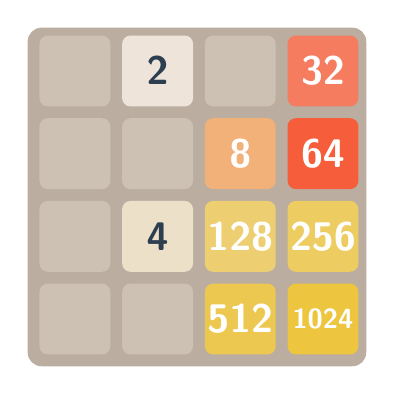
\begin{tikzpicture}
\fill[boardbg,rounded corners=5pt](-0.15,-0.15)rectangle(4.15,4.15);
\fill[emptycell,rounded corners=3pt](0,0)rectangle(0.9,0.9);
\fill[emptycell,rounded corners=3pt](1.05,0)rectangle(1.95,0.9);
\fill[tile512,rounded corners=3pt](2.1,0)rectangle(3,0.9);
\node[font=\bfseries\small,text=white]at(2.55,0.45){512};
\fill[tile1024,rounded corners=3pt](3.15,0)rectangle(4.05,0.9);
\node[font=\bfseries\tiny,text=white]at(3.6,0.45){1024};
\fill[emptycell,rounded corners=3pt](0,1.05)rectangle(0.9,1.95);
\fill[tile4,rounded corners=3pt](1.05,1.05)rectangle(1.95,1.95);
\node[font=\bfseries\small,text=darktext]at(1.5,1.5){4};
\fill[tile128,rounded corners=3pt](2.1,1.05)rectangle(3,1.95);
\node[font=\bfseries\small,text=white]at(2.55,1.5){128};
\fill[tile256,rounded corners=3pt](3.15,1.05)rectangle(4.05,1.95);
\node[font=\bfseries\small,text=white]at(3.6,1.5){256};
\fill[emptycell,rounded corners=3pt](0,2.1)rectangle(0.9,3);
\fill[emptycell,rounded corners=3pt](1.05,2.1)rectangle(1.95,3);
\fill[tile8,rounded corners=3pt](2.1,2.1)rectangle(3,3);
\node[font=\bfseries\small,text=white]at(2.55,2.55){8};
\fill[tile64,rounded corners=3pt](3.15,2.1)rectangle(4.05,3);
\node[font=\bfseries\small,text=white]at(3.6,2.55){64};
\fill[emptycell,rounded corners=3pt](0,3.15)rectangle(0.9,4.05);
\fill[tile2,rounded corners=3pt](1.05,3.15)rectangle(1.95,4.05);
\node[font=\bfseries\small,text=darktext]at(1.5,3.6){2};
\fill[emptycell,rounded corners=3pt](2.1,3.15)rectangle(3,4.05);
\fill[tile32,rounded corners=3pt](3.15,3.15)rectangle(4.05,4.05);
\node[font=\bfseries\small,text=white]at(3.6,3.6){32};
\end{tikzpicture}}
\end{minipage}%
\hfill
\begin{minipage}[t]{0.53\linewidth}
\footnotesize
Slide tiles in 4 directions. Equal tiles merge and double. Reach \textbf{2048} to win.
\vspace{3pt}

\textbf{Challenges:}
\begin{itemize}[nosep,leftmargin=9pt,itemsep=1pt]
  \item[$\bullet$] ${\sim}10^{19}$ reachable board states
  \item[$\bullet$] Sparse, delayed reward signal
  \item[$\bullet$] Stochastic tile spawns (2 or 4)
  \item[$\bullet$] 100--1,000$+$ steps per episode
  \item[$\bullet$] Up to 4 invalid actions per state
\end{itemize}
\end{minipage}

\vspace{5pt}
\footnotesize\textbf{MDP Formulation:}
\vspace{2pt}

\renewcommand{\arraystretch}{1.2}
{\footnotesize\begin{tabular}{@{}>{\bfseries\color{sectioncolor}}l@{\;\;}p{0.72\linewidth}@{}}
$\mathcal{S}$ & $4{\times}4$ board $\to$ 16-ch binary tensor $\{0,1\}^{16\times4\times4}$\\
$\mathcal{A}$ & \{UP, RIGHT, DOWN, LEFT\}; invalid masked to $-\infty$\\
$\mathcal{R}$ & $\Delta$score $+$ milestones: $+50$@256, $+100$@512, $+200$@1024\\
$\gamma$ & 0.99 (long-horizon credit assignment)\\
\end{tabular}}
\end{sectionbox}

% ── Design of Experiments ─────────────────────────────────────────────
\begin{sectionbox}[Design of Experiments]{info}
\footnotesize
\textbf{Research Question:} Can LLM-guided RLVR (GRPO: Group Relative Policy Optimization) match classical RL agents on a structured combinatorial game under equivalent compute constraints?

\vspace{4pt}
\textbf{Agent Lineup: 6 Classical $+$ 2 LLM:}
\vspace{2pt}

\renewcommand{\arraystretch}{1.15}
{\footnotesize\begin{tabular}{@{}>{\bfseries}l l l@{}}
\rowcolor{headerbg!10}
Agent & Category & Impl. \\
\midrule
DQN            & Off-policy, value-based & Custom PyTorch \\
SAC (Discrete) & Off-policy, max-entropy & Custom PyTorch \\
QR-DQN         & Off-policy, distributional & SB3 \\
PPO            & On-policy, clipped & SB3 \\
A2C            & On-policy, actor-critic & SB3 \\
Semi-grad SARSA& On-policy, linear FA & Custom NumPy \\
GRPO 0.5B      & LLM-RLVR & trl \\
GRPO 1.5B      & LLM-RLVR & trl \\
\end{tabular}}

\vspace{5pt}
\textbf{Shared Experimental Controls:}
\begin{itemize}[nosep,leftmargin=13pt,itemsep=2pt]
  \item All deep agents: \textbf{identical CNN backbone} (3-layer, 330K params)
  \item Same shaped reward function and 2048 gym environment
  \item Invalid action masking applied uniformly across all agents
  \item Evaluation: last 100 episodes + unlimited ``Hunt'' (best-of-N) mode
\end{itemize}

\vspace{4pt}
\textbf{Training Protocol:}
\vspace{2pt}

{\footnotesize\begin{tabular}{@{}>{\bfseries}l l l@{}}
Classical (1M ckpt): & 1M env steps & intermediate eval \\
Classical (5M ckpt): & 5M env steps & $\approx$2\,hrs, RTX 4060 \\
GRPO:                & 300 prompts $\times$ 4 & $\approx$12\,hrs, RTX 4060 \\
\end{tabular}}

\vspace{4pt}
\begin{calloutbox}[info]
{\footnotesize\textbf{CNN Backbone} (shared): Conv(16, $3{\times}3$) $\to$ Conv(32, $3{\times}3$) $\to$ Conv(64, $3{\times}3$) $\to$ FC(512) $\to$ Q(4). Input: 16-channel binary encoding of tile values. \textbf{330K params}. Score differences reflect the \emph{learning algorithm only}.}
\end{calloutbox}
\end{sectionbox}

\sectiontitle{Algorithms}

% ── DQN ───────────────────────────────────────────────────────────────
\begin{sectionbox}[DQN $\bigstar$ Best Performer \hfill \customtag]{dqncolor}
\begin{minipage}[t]{0.48\linewidth}
\begin{parambox}
\footnotesize\textbf{Off-policy, value-based}\par\vspace{3pt}
\renewcommand{\arraystretch}{1.15}
\begin{tabular}{@{}l l@{}}
Buffer:    & 100K transitions \\
Batch:     & 64 \\
$\varepsilon$: & $1.0 \to 0.01$ / 100K \\
Target:    & hard sync / 1K \\
LR:        & $10^{-4}$ (Adam) \\
Grad clip: & 1.0 \\
\end{tabular}
\end{parambox}
\end{minipage}%
\hfill
\begin{minipage}[t]{0.48\linewidth}
\begin{codebox}
{\scriptsize\ttfamily\textbf{DQN Update:}\\
1. Sample $(s,a,r,s')$ from $\mathcal{B}$\\
2. Mask invalid $a'$ to $-\infty$\\
3. $y \gets r + \gamma\max_{a'}Q_{\bar\theta}(s',a')$\\
4. $\mathcal{L} \gets \text{SmoothL1}(Q_\theta,\,y)$\\
5. $\theta \gets \theta - \alpha\nabla\mathcal{L}$\\
6. Sync $\bar\theta \gets \theta$ every $C$ steps}
\end{codebox}
\end{minipage}
\vspace{3pt}
\begin{calloutbox}[dqncolor]
{\footnotesize\textbf{Why DQN wins:} Replay buffer revisits high-tile transitions thousands of times. States with tile $\geq512$ ($<$0.1\% of all steps) are repeatedly replayed. On-policy methods see each transition \textbf{exactly once}: no second chance.}
\end{calloutbox}
\end{sectionbox}

% ── SAC ───────────────────────────────────────────────────────────────
\begin{sectionbox}[SAC (Discrete) \hfill \customtag]{dqncolor}
\begin{minipage}[t]{0.48\linewidth}
\begin{parambox}
\footnotesize\textbf{Off-policy, max-entropy}\par\vspace{2pt}
$J(\pi)=\textstyle\sum_t\mathbb{E}[r_t+\alpha\mathcal{H}[\pi(\cdot|s_t)]]$\par\vspace{3pt}
\renewcommand{\arraystretch}{1.15}
\begin{tabular}{@{}l l@{}}
Buffer:       & 200K transitions \\
Batch:        & 256 \\
Polyak $\tau$:& 0.005 \\
LR:           & $10^{-4}$ (Adam) \\
Warmup:       & 10K steps \\
Target ent.:  & $0.4\log|\mathcal{A}|$ \\
\end{tabular}
\end{parambox}
\end{minipage}%
\hfill
\begin{minipage}[t]{0.48\linewidth}
\begin{codebox}
{\scriptsize\ttfamily\textbf{SAC Update:}\\
1. Sample $(s,a,r,s')$ from $\mathcal{B}$\\
2. Mask invalid actions in $\pi$\\
3. $y\gets r+\gamma(Q_{\min}-\alpha\log\pi)$\\
4. Update twin $Q_1, Q_2$ critics\\
5. Update $\pi$ via entropy objective\\
6. Auto-tune $\alpha$ to target entropy}
\end{codebox}
\end{minipage}
\vspace{3pt}
\begin{calloutbox}[dqncolor]
{\footnotesize Max-entropy bonus diversifies tile placement but over-explores in sparse-reward episodes. Soft Polyak update ($\tau{=}0.005$) slows critic convergence vs.\ DQN's hard sync. Avg score: \textbf{1,255}, $6\times$ below DQN.}
\end{calloutbox}
\end{sectionbox}

%═══════════════════════════════════════ COLUMN 2 ══════════════════════

% ── PPO ───────────────────────────────────────────────────────────────
\begin{sectionbox}[PPO (MaskablePPO) \hfill \sbtag]{info}
\begin{minipage}[t]{0.48\linewidth}
\begin{parambox}
\footnotesize\textbf{On-policy, clipped actor-critic}\par\vspace{3pt}
\renewcommand{\arraystretch}{1.15}
\begin{tabular}{@{}l l@{}}
Rollout: & 2048 steps $\times$ 8 envs \\
Batch:   & 64 \\
Epochs:  & 10 per rollout \\
LR:      & $3{\times}10^{-4}$ \\
GAE:     & $\lambda{=}0.95$ \\
Clip:    & $\epsilon{=}0.2$ \\
Entropy: & $c_e{=}0.01$ \\
\end{tabular}
\end{parambox}
\end{minipage}%
\hfill
\begin{minipage}[t]{0.48\linewidth}
\begin{codebox}
{\scriptsize\ttfamily\textbf{PPO Update:}\\
1. Collect rollout ($T$ steps, 8 envs)\\
2. Compute GAE adv.\ $\hat{A}$\\
3. $r_t(\theta)=\pi_\theta/\pi_{\text{old}}$\\
4. $\mathcal{L}=\min(r_t\hat{A},\text{clip}(r_t)\hat{A})$\\
5. Update $\theta$ for $K{=}10$ epochs\\
6. \textbf{Discard all rollout data}}
\end{codebox}
\end{minipage}
\vspace{3pt}
\begin{calloutbox}[danger]
{\footnotesize\textbf{Why PPO fails:} Each ${\sim}400$-step episode used \textbf{once} then discarded. Effective discount $\gamma^{400}{\approx}0.018$ kills gradient signal for early moves. Score \textbf{drops 12\%} from 1M$\to$5M steps: active policy degradation.}
\end{calloutbox}
\end{sectionbox}

% ── A2C ───────────────────────────────────────────────────────────────
\begin{sectionbox}[A2C \hfill \sbtag]{info}
\begin{minipage}[t]{0.48\linewidth}
\begin{parambox}
\footnotesize\textbf{On-policy, actor-critic}\par\vspace{1pt}
No clipping; single gradient step.\par\vspace{3pt}
\renewcommand{\arraystretch}{1.15}
\begin{tabular}{@{}l l@{}}
n\_steps: & 5 \\
LR:       & $7{\times}10^{-4}$ \\
$c_e$:    & 0.01 \\
$c_v$:    & 0.5 \\
\end{tabular}\par\vspace{3pt}
$\mathcal{L}=-\mathbb{E}[\log\pi\hat{A}]$
$\quad+0.5\|R{-}V\|^2-0.01\mathcal{H}$
\end{parambox}
\end{minipage}%
\hfill
\begin{minipage}[t]{0.48\linewidth}
\begin{codebox}
{\scriptsize\ttfamily\textbf{A2C Update:}\\
1. Collect 5-step rollout\\
2. $\hat{A} \gets R - V(s)$\\
3. $\mathcal{L}_\pi \gets -\log\pi\hat{A}$\\
4. $\mathcal{L}_v \gets 0.5\|R{-}V\|^2$\\
5. $\mathcal{L}\gets\mathcal{L}_\pi+\mathcal{L}_v-c_e\mathcal{H}$\\
6. Single gradient step on $\mathcal{L}$}
\end{codebox}
\end{minipage}
\vspace{3pt}
\begin{calloutbox}[info]
{\footnotesize 5-step bootstrap limits credit in 400-step episodes. Yet \textbf{beats PPO by +982 avg}: faster LR ($7{\times}10^{-4}$) and synchronous updates converge better early on. Simpler objective = more stable gradient.}
\end{calloutbox}
\end{sectionbox}

% ── QR-DQN ────────────────────────────────────────────────────────────
\begin{sectionbox}[QR-DQN (Distributional) \hfill \sbtag]{info}
\begin{minipage}[t]{0.48\linewidth}
\begin{parambox}
\footnotesize\textbf{Off-policy, distributional}\par\vspace{1pt}
Learns full return distribution via $N{=}50$ quantiles rather than $\mathbb{E}[Q]$.\par\vspace{3pt}
\renewcommand{\arraystretch}{1.15}
\begin{tabular}{@{}l l@{}}
Buffer:  & 100K \\
$N$:     & 50 quantiles \\
Output:  & $4{\times}50{=}200$ values \\
LR:      & $10^{-4}$ \\
Target:  & sync / 1K steps \\
\end{tabular}
\end{parambox}
\end{minipage}%
\hfill
\begin{minipage}[t]{0.48\linewidth}
\begin{codebox}
{\scriptsize\ttfamily\textbf{QR-DQN Update:}\\
1. Sample $(s,a,r,s')$ from $\mathcal{B}$\\
2. For each quantile $\tau_i$:\\
\;\;$\delta_{ij}=r+\gamma\theta_j(s')-\theta_i(s)$\\
3. $\mathcal{L}=\textstyle\sum_i\rho_{\tau_i}^{\kappa}(\delta_{ij})$\\
4. $a^*=\arg\max_a\frac{1}{N}\sum_i\theta_i$}
\end{codebox}
\end{minipage}
\vspace{3pt}
\begin{calloutbox}[danger]
{\footnotesize Action selection by $\text{mean}(Q)$ is \textbf{identical to DQN}. Distributional modeling provides no behavioral gain. Quantile regression on non-stationary 2048 targets causes instability: score \textbf{degrades $-9\%$} from 1M$\to$5M.}
\end{calloutbox}
\end{sectionbox}

% ── SARSA ─────────────────────────────────────────────────────────────
\begin{sectionbox}[Semi-gradient SARSA (S\&B Alg.\ 10.1) \hfill \numpytag]{success}
\begin{minipage}[t]{0.48\linewidth}
\begin{parambox}
\footnotesize\textbf{On-policy, linear FA (no neural net!)}\par\vspace{2pt}
$\hat{q}(s,a,\mathbf{w})=\mathbf{w}_a^\top\phi(s)$\par\vspace{1pt}
$\mathbf{w}\in\mathbb{R}^{4\times30}=\textbf{120 params}$\par\vspace{3pt}
\renewcommand{\arraystretch}{1.1}
\begin{tabular}{@{}l l@{}}
$\alpha$:            & $10^{-3}$ \\
$\varepsilon$ decay: & 0.99995/step \\
$\varepsilon_{\min}$:& 0.05 \\
\end{tabular}\par\vspace{3pt}
\textbf{30-dim $\phi(s)$ (S\&B \S9.5):}
\begin{itemize}[nosep,leftmargin=9pt,itemsep=0pt]
\item[$\cdot$] $\log_2(\text{tile})$ values $\times16$
\item[$\cdot$] Empty cell ratio, merge potential
\item[$\cdot$] Monotonicity L/R/U/D ($\times4$)
\item[$\cdot$] Corner bonus, smoothness ($\times2$)
\item[$\cdot$] Snake pattern, edge sum ($\times2$)
\item[$\cdot$] Bias/interaction terms ($\times4$)
\end{itemize}
\end{parambox}
\end{minipage}%
\hfill
\begin{minipage}[t]{0.48\linewidth}
\begin{codebox}
{\scriptsize\ttfamily\textbf{SARSA Update (Alg 10.1):}\\
1. Observe $s$, choose $a$ ($\varepsilon$-greedy)\\
2. Take $a$, observe $r, s'$\\
3. Choose $a'$ ($\varepsilon$-greedy on $s'$)\\
4. $\delta\gets r+\gamma\hat{q}(s',a')-\hat{q}(s,a)$\\
5. $\mathbf{w}_a\gets\mathbf{w}_a+\alpha\delta\phi(s)$\\
6. $s\gets s',\; a\gets a'$}
\end{codebox}
\vspace{4pt}
\begin{calloutbox}[success]
{\footnotesize\textbf{120 params beats 330K+!} Game-specific inductive bias (monotonicity, snake) outperforms CNN on on-policy data. Validates S\&B \S9.5.}
\end{calloutbox}
\end{minipage}
\end{sectionbox}

% ── GRPO ──────────────────────────────────────────────────────────────
\begin{sectionbox}[GRPO: Group Relative Policy Optimization \hfill \grpotag]{purple}
\footnotesize
\textbf{GRPO} (Group Relative Policy Optimization, DeepSeek-R1, 2025): fine-tunes \textbf{Qwen2.5-0.5B / 1.5B} via verifiable rewards \emph{without} a critic. Board $\to$ ASCII text $\to$ chain-of-thought reasoning $\to$ action token. No replay buffer.

\vspace{4pt}
\begin{minipage}[t]{0.48\linewidth}
\begin{parambox}
\footnotesize
\textbf{Group-normalized advantage:}\par\vspace{2pt}
$$\hat{A}_i = \frac{r_i - \mu_G}{\sigma_G + \epsilon},\quad G{=}4$$\par\vspace{1pt}
\textbf{3-stage reward scheduling:}
\begin{enumerate}[nosep,leftmargin=14pt,itemsep=2pt]
  \item Format compliance (XML tags)
  \item Game reward ($\Delta$score)
  \item Thinking quality (token bonus)
\end{enumerate}\par\vspace{3pt}
\textbf{Compute cost:} 4 LLM forward passes per training step. 300 prompts $\approx$ \textbf{12 hrs} on RTX 4060 vs.\ \textbf{2 hrs} for 5M classical steps.
\end{parambox}
\end{minipage}%
\hfill
\begin{minipage}[t]{0.48\linewidth}
\begin{codebox}
{\scriptsize\ttfamily\textbf{GRPO Update:}\\
1. Sample $G{=}4$ completions\\
2. Score each: $r_i\gets$ verifier\\
3. $\hat{A}_i=(r_i-\mu_G)/\sigma_G$\\
4. $\mathcal{L}=-\sum_i\hat{A}_i\log\pi_\theta$\\
\quad$-\beta\,\text{KL}(\pi_\theta\|\pi_{\text{ref}})$\\
5. Update $\theta$; repeat for next prompt}
\end{codebox}
\vspace{4pt}
\begin{calloutbox}[purple]
{\footnotesize LLM sees $1{,}200$ states vs.\ DQN's 5M. Produces \textbf{interpretable CoT} per move. $3\times$ model $\to$ $3.3\times$ score: \textbf{scaling is the lever}.}
\end{calloutbox}
\end{minipage}

\vspace{5pt}
% ── CoT example + spatial failure ─────────────────────────────────
\noindent\begin{minipage}[t]{0.50\linewidth}
\begin{codebox}
{\scriptsize\ttfamily
\textbf{Input (Qwen2.5-1.5B, move 41):}\\
Board: [[0,0,4,8],[0,4,16,32],\\
\quad\quad\;\;[0,0,64,128],[0,0,0,256]]\\
Max tile: 256 | Score: 956\\[3pt]
\textbf{<think>}\\
256 anchored bottom-right -- good.\\
Gradient: 128, 64, 32, 16 intact\\
along right/bottom edges.\\
RIGHT merges 4+4 in row 1 (+8).\\
Avoids scattering corner tile.\\
\textbf{</think>}\\
\textbf{<answer>}RIGHT\textbf{</answer>}\quad\color{success}{$\checkmark$ +8}}
\end{codebox}
\end{minipage}%
\hfill
\begin{minipage}[t]{0.47\linewidth}
\begin{calloutbox}[danger]
{\footnotesize\textbf{\color{danger}Spatial Failure (0.5B):}\\[2pt]
Board: \texttt{[[0,4,0,0],[4,0,8,0],...]}\\[2pt]
Model: \textit{``4 at [0][1] and [1][0] are adjacent -- LEFT merges them into 8''}\\[2pt]
\textbf{Reality:} they are in different rows. LEFT moves each to col 0 independently. No merge occurs.\\[2pt]
Root cause: LLM pattern-matches on \textbf{token proximity}, not grid geometry. Cannot mentally simulate a slide.}
\end{calloutbox}
\end{minipage}
\end{sectionbox}

%═══════════════════════════════════════ COLUMN 3 ══════════════════════

% ── Training Curves ───────────────────────────────────────────────────
\begin{sectionbox}[Training Curves (5M Steps)]{sectioncolor}
\noindent\begin{minipage}[t]{0.48\linewidth}
\centering
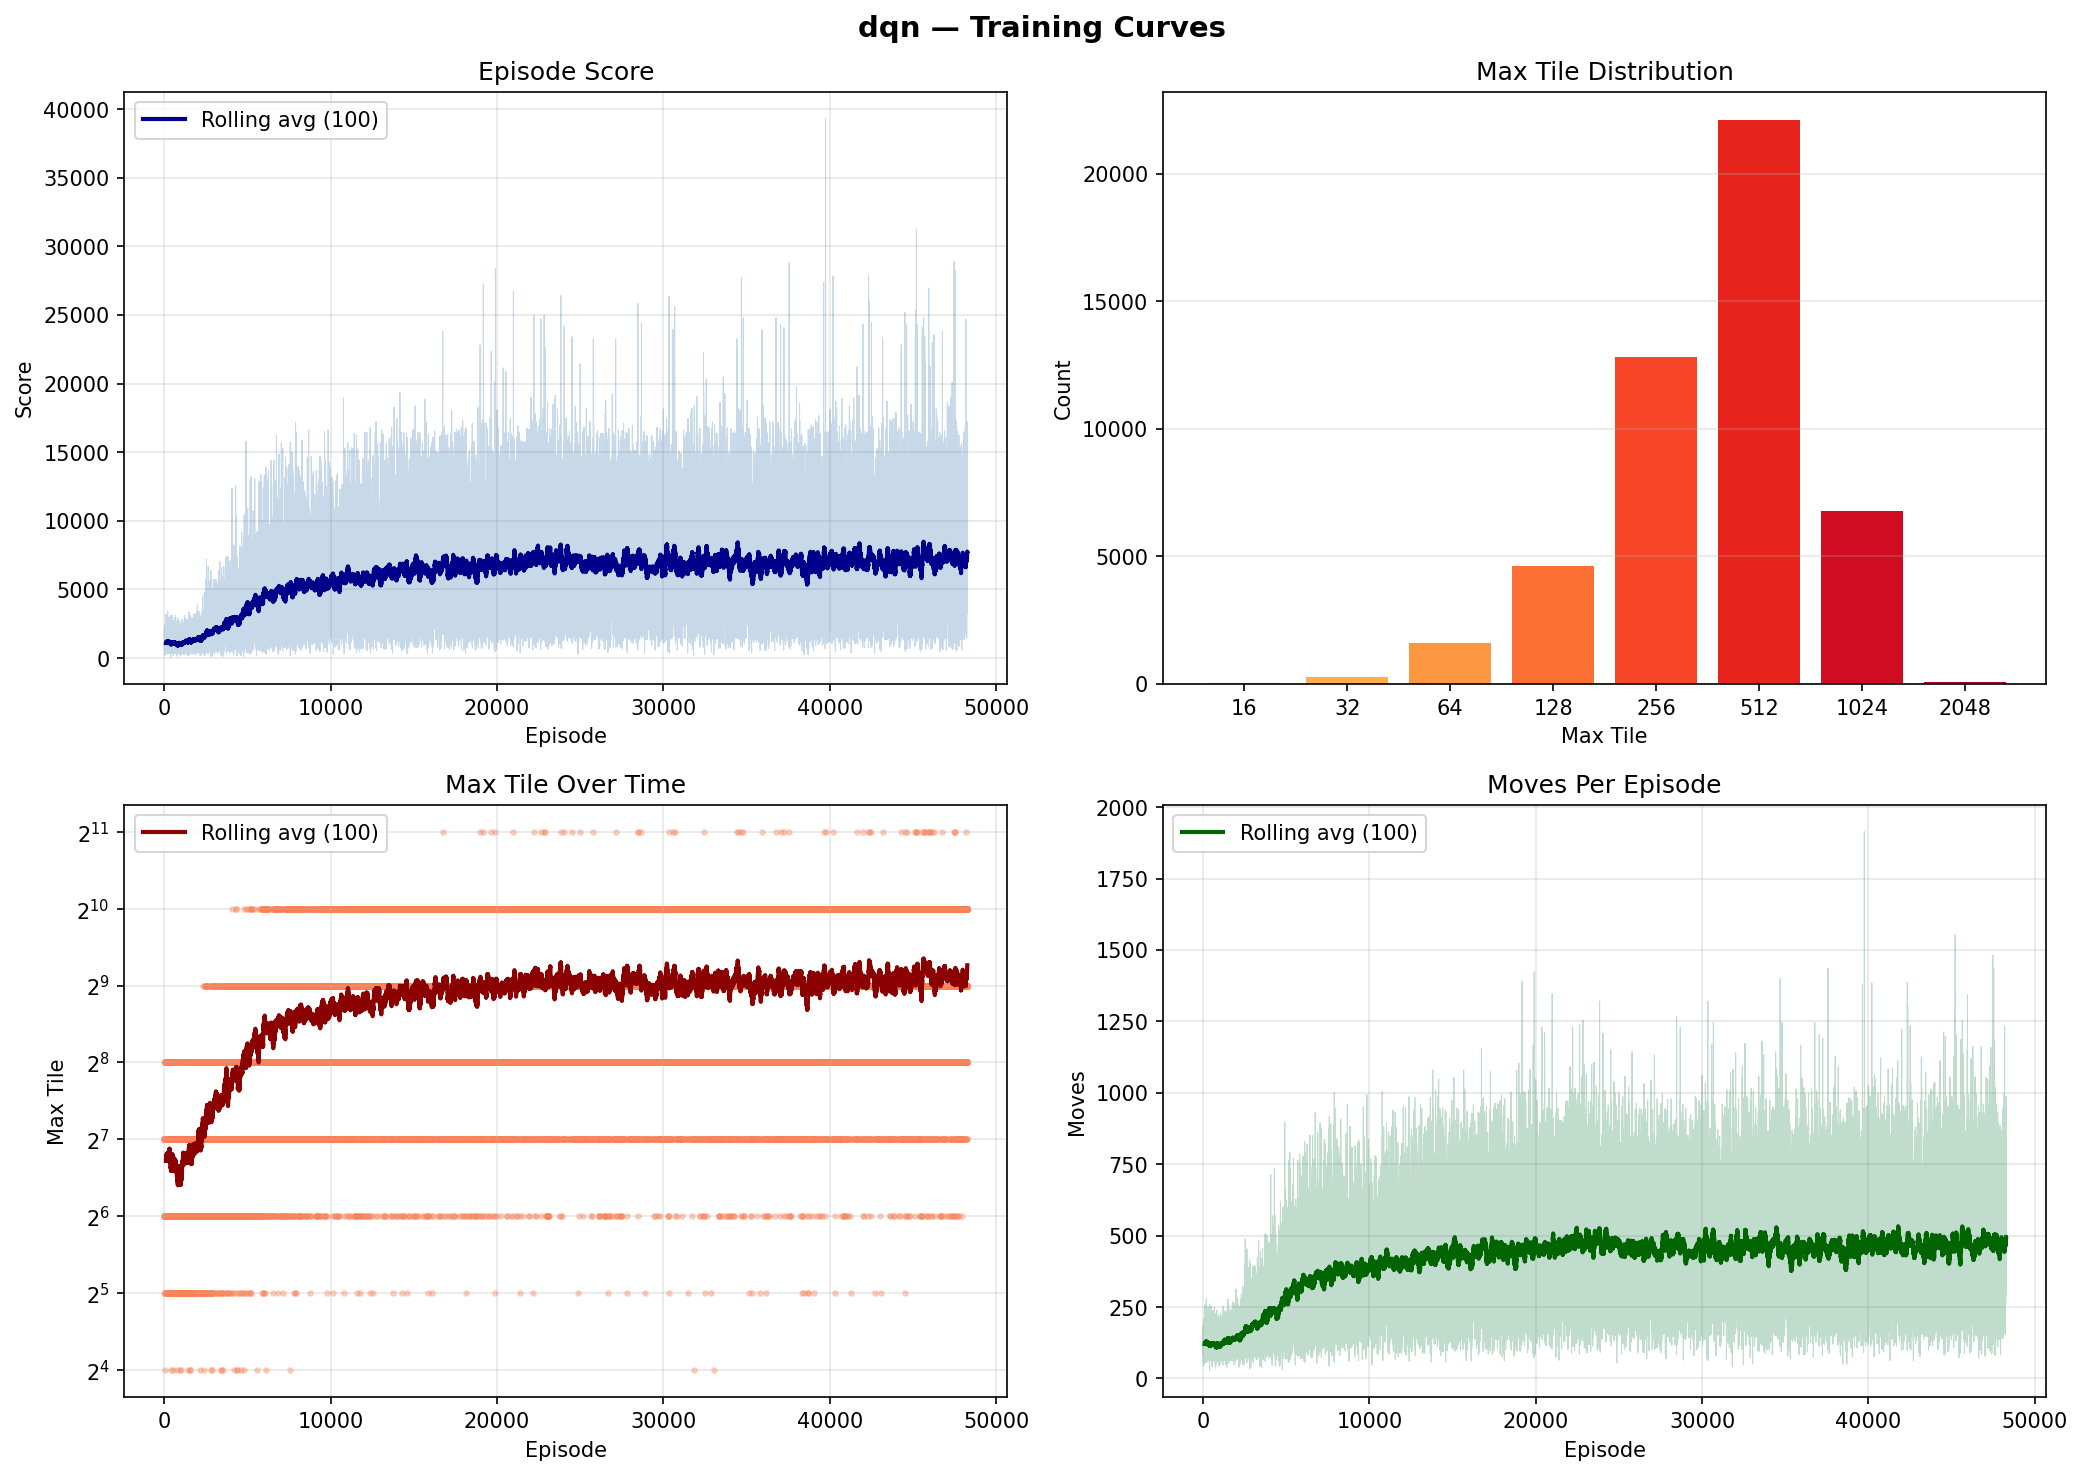
\includegraphics[width=\linewidth]{fig_dqn_5m.png}\\[1pt]
{\footnotesize\bfseries\color{dqncolor} DQN: avg 7,744 $\bigstar$}
\end{minipage}%
\hfill
\begin{minipage}[t]{0.48\linewidth}
\centering
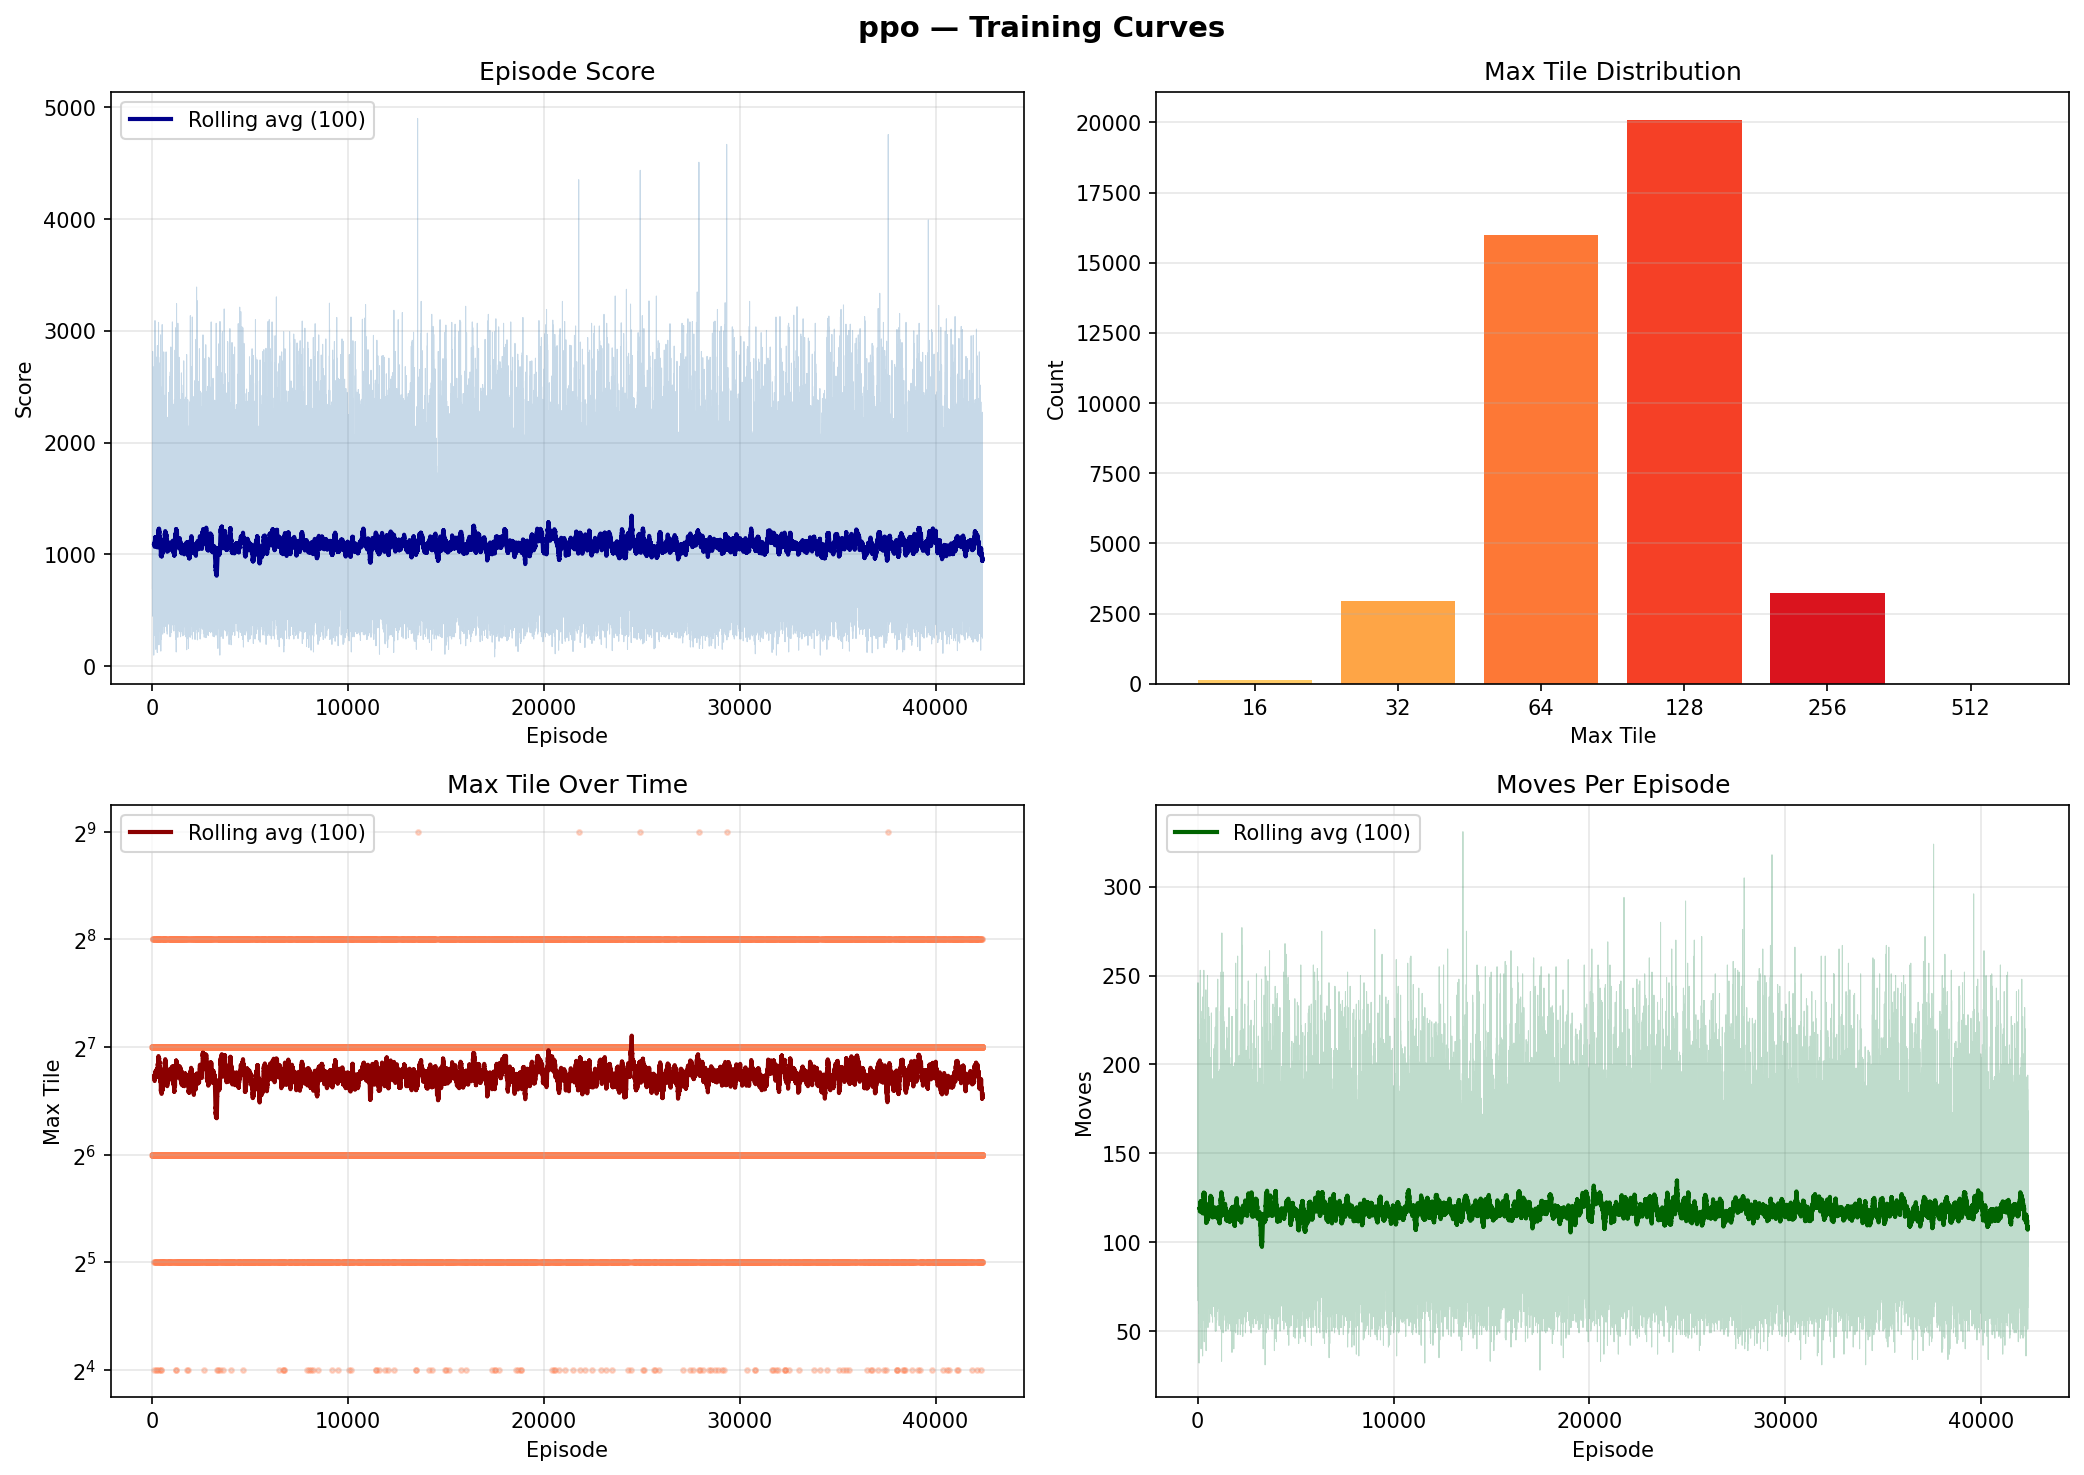
\includegraphics[width=\linewidth]{fig_ppo_5m.png}\\[1pt]
{\footnotesize\bfseries\color{danger} PPO: avg 962 $\downarrow$ (degrades!)}
\end{minipage}\par\vspace{3pt}
\noindent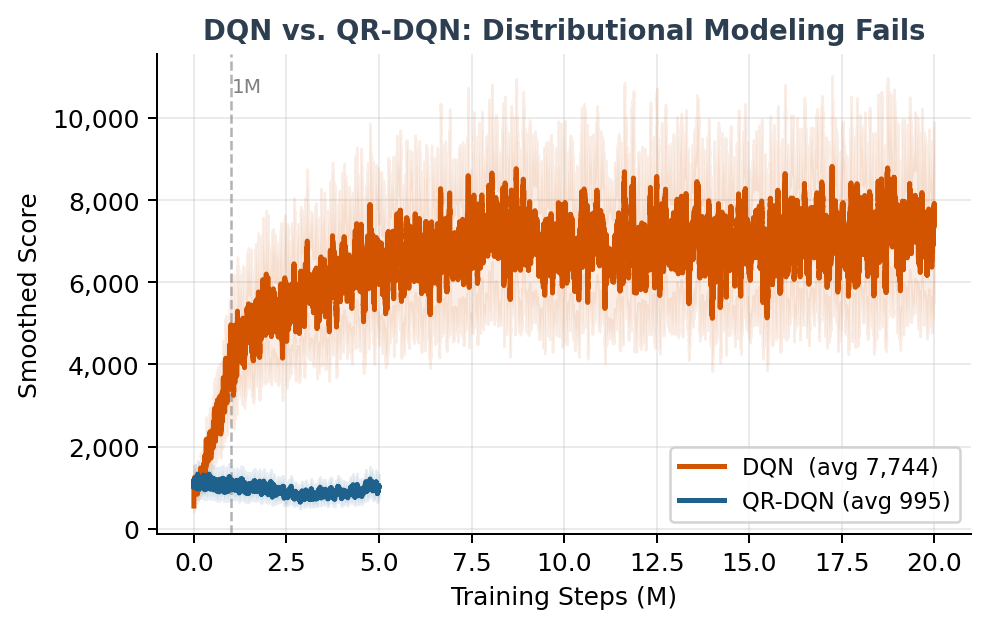
\includegraphics[width=\linewidth]{fig_dqn_vs_qrdqn.png}\par\vspace{1pt}
{\footnotesize\centering\color{darktext!65}
SARSA: 2,456\enspace\textbar\enspace
SAC: 1,255\enspace\textbar\enspace
A2C: 1,944\enspace(see table below)}
\end{sectionbox}

% ── Results Table ─────────────────────────────────────────────────────
\begin{sectionbox}[Final Performance (5M Steps)]{accent}
\renewcommand{\arraystretch}{1.2}
\resizebox{\linewidth}{!}{%
\footnotesize
\begin{tabular}{@{}>{\bfseries}l r r r r r l@{}}
\toprule
\rowcolor{headerbg!10}
\textbf{Agent} & \textbf{Avg Score} & \textbf{Max Score} & \textbf{Max Tile} & \textbf{512+ Rate} & \textbf{Params} & \textbf{Impl.} \\
\midrule
\rowcolor{dqnlight}
DQN $\bigstar$  & \color{dqncolor}{\textbf{7,744}}  & \color{dqncolor}{\textbf{39,314}} & \color{dqncolor}{\textbf{2048}} & \color{dqncolor}{\textbf{76\%}} & 330K   & Custom \\
SARSA           & 2,456 & 11,436 & 1024 & 6\%       & \color{success}{\textbf{120}} & NumPy \\
\rowcolor{purplelight}
GRPO 1.5B       & \color{purple}{2,348} & 2,348 & \color{purple}{256} & 0\% & 1.8B  & trl \\
A2C             & 1,944 & 9,640  & 1024 & 6\%       & 330K   & SB3 \\
GRPO 0.5B       & 1,816 & 1,816  & 128  & 0\%       & 494M   & trl \\
SAC             & 1,255 & 7,882  & 512  & $<$1\%    & 330K   & Custom \\
QR-DQN          & 995   & 5,176  & 512  & $<$1\%    & 430K   & SB3 \\
\rowcolor{dangerlight}
PPO             & \color{danger}{962} & 4,900 & 512 & $<$1\%  & 330K   & SB3 \\
\bottomrule
\end{tabular}}
\end{sectionbox}

% ── Scaling ───────────────────────────────────────────────────────────
\begin{sectionbox}[Sample Efficiency: 1M $\to$ 5M Steps]{info}
\noindent
\includegraphics[width=\linewidth]{fig_sample_efficiency.png}
\end{sectionbox}

% ── Hunt Mode ─────────────────────────────────────────────────────────
\begin{sectionbox}[Hunt Mode: Can Any Agent Reach 2048?]{sectioncolor}
\footnotesize
Unlimited attempts with $\varepsilon{=}0.05$ exploration. Runs until tile 2048 reached or 3K attempts.
\vspace{3pt}

\renewcommand{\arraystretch}{1.2}
\resizebox{\linewidth}{!}{%
\footnotesize
\begin{tabular}{@{}>{\bfseries}l r r r l@{}}
\toprule
\rowcolor{headerbg!10}
\textbf{Agent} & \textbf{Attempts} & \textbf{Best Tile} & \textbf{Best Score} & \textbf{Verdict} \\
\midrule
\rowcolor{dqnlight}
DQN $\bigstar$ & 3,902 & \color{dqncolor}{\textbf{2048}} & \color{dqncolor}{\textbf{21,572}} & \color{dqncolor}{\textbf{Only success}} \\
SARSA          & 3,000 & 1024 & 12,300 & Closest (120 params!) \\
A2C            & 3,000 & 512  & 7,844  & Stalls post-512 \\
SAC            & 3,000 & 256  & 3,648  & Entropy hurts late \\
\rowcolor{dangerlight}
PPO            & 193   & \color{danger}{64} & \color{danger}{520} & \color{danger}{Collapses early} \\
\bottomrule
\end{tabular}}
\vspace{3pt}
\begin{calloutbox}[dqncolor]
{\footnotesize\textbf{DQN is the only agent to reach 2048} in 3,902 unlimited attempts (0.026\% rate). Replay buffer is the decisive factor even in best-case conditions. SARSA reaches 1024 with 120 params; PPO degrades to tile 64 under hunt pressure.}
\end{calloutbox}
\end{sectionbox}

% ── Classical vs RLVR ─────────────────────────────────────────────────
\sectiontitle{Classical RL vs.\ RLVR}

\begin{sectionbox}[Head-to-Head Comparison]{accent}
\renewcommand{\arraystretch}{1.2}
\resizebox{\linewidth}{!}{%
\footnotesize
\begin{tabular}{@{}>{\bfseries}l l l@{}}
\toprule
\rowcolor{headerbg!10}
\textbf{Dimension} & \textbf{Classical RL} & \textbf{LLM-RLVR (GRPO)} \\
\midrule
Avg Score     & \color{dqncolor}{\textbf{7,744}} (DQN) & 2,348 (1.5B) \\
Max Tile      & \color{dqncolor}{\textbf{2048}} (DQN) & 256 (1.5B) \\
\rowcolor{purplelight}
Parameters    & 120 -- 430K & \color{purple}{\textbf{494M -- 1.8B}} \\
\rowcolor{dqnlight}
Inference     & \color{dqncolor}{\textbf{$<$4\,ms/move}} & 1,500\,ms/move \\
Training data & 5M env steps & 300 prompts \\
\rowcolor{purplelight}
Interpretable & No (black box) & \color{purple}{\textbf{Yes: chain-of-thought}} \\
Observation   & Tensor $16{\times}4{\times}4$ & ASCII board text \\
Action space  & Integer $\{0,1,2,3\}$ & Natural language token \\
\bottomrule
\end{tabular}}

\vspace{4pt}
{\footnotesize
\textbf{Score gap:} DQN replays 5M transitions; GRPO sees 1,200 board states. Tensor input is dense information; ASCII forces tokenization overhead.

\textbf{RLVR strength:} Each GRPO move is paired with an inspectable reasoning trace. Classical agents are complete black boxes with no explainability.

\textbf{Scaling law:} $0.5\text{B}\to1.5\text{B}$ ($3\times$ params) $\to$ $3.3\times$ score. LLM model size is the primary performance lever.}\par\vspace{4pt}
\noindent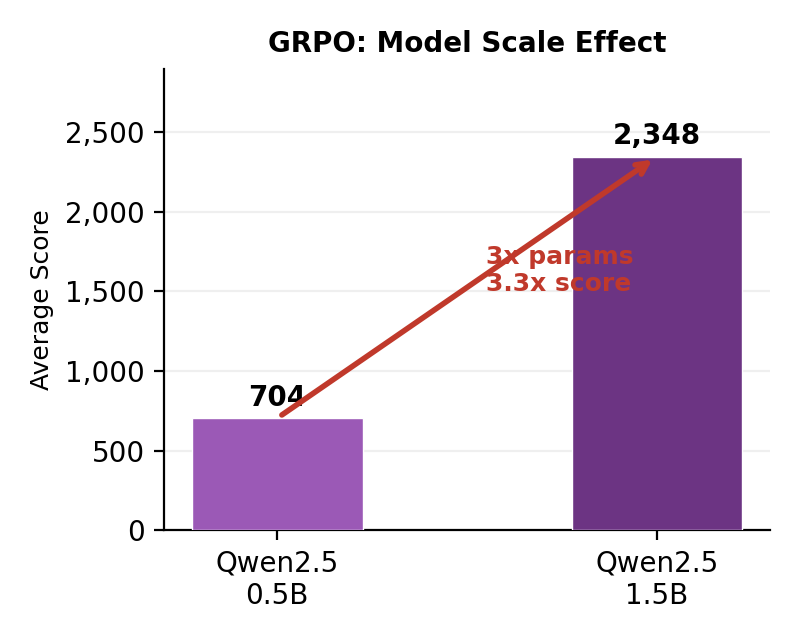
\includegraphics[width=\linewidth]{fig_grpo_scaling.png}
\end{sectionbox}

% ── Key Findings ──────────────────────────────────────────────────────
\sectiontitle{Key Findings}

\begin{highlightbox}[dqncolor]
\footnotesize\textbf{\color{dqncolor}1.\enspace Off-policy replay is decisive.}\enspace
DQN's 100K replay buffer (S\&B \S8.2) recycles rare high-tile transitions that on-policy methods see only once. PPO score $=962$; DQN $=7{,}744$ on identical CNN. Replay gap $=8\times$.
\end{highlightbox}

\begin{highlightbox}[success]
\footnotesize\textbf{\color{success}2.\enspace 120 params beats 330K+ at sample efficiency.}\enspace
Semi-gradient SARSA with hand-crafted features (monotonicity, snake, corner) outperforms all deep on-policy agents. Validates S\&B \S9.5: strong inductive bias beats raw capacity when data is scarce.
\end{highlightbox}

\begin{highlightbox}[danger]
\footnotesize\textbf{\color{danger}3.\enspace More training actively hurts on-policy agents.}\enspace
PPO $-12\%$ and QR-DQN $-9\%$ from 1M$\to$5M. PPO develops degenerate tile-sliding loops; QR-DQN collapses under distributional overfitting. On-policy methods \emph{unlearn} good behavior.
\end{highlightbox}

\begin{highlightbox}[purple]
\footnotesize\textbf{\color{purple}4.\enspace LLM scale drives RLVR performance.}\enspace
$3\times$ parameters ($0.5\text{B}\to1.5\text{B}$) $\to$ $3.3\times$ avg score. GRPO uniquely produces \emph{interpretable} per-move rationale. At larger scale (3B+), GRPO is the strongest candidate to close the gap.
\end{highlightbox}

% ── Future Work ───────────────────────────────────────────────────────
\begin{sectionbox}[Future Work]{sectioncolor}
\footnotesize
\begin{itemize}[nosep,leftmargin=13pt,itemsep=3pt]
  \item[\color{dqncolor}$\triangleright$] \textbf{Replay buffer ablation:} vary DQN buffer (10K/50K/100K/500K) to quantify exactly how much replay drives the $8\times$ PPO gap
  \item[\color{dqncolor}$\triangleright$] \textbf{Prioritized Experience Replay (PER):} over-sample rare high-tile transitions; directly motivated by Key Finding 1
  \item[\color{purple}$\triangleright$] \textbf{Spatial board encoding for GRPO:} replace list-of-lists with labeled ASCII grid to test if spatial failures decrease
  \item[\color{purple}$\triangleright$] \textbf{Extended GRPO training:} 300 $\to$ 1K+ prompts on Colab A100 (free tier); directly tests whether the scaling law continues
  \item[\color{success}$\triangleright$] \textbf{Multi-seed eval} ($n{=}5$) for all classical agents to establish statistical significance of SARSA vs. deep on-policy gap
\end{itemize}
\end{sectionbox}

{\scriptsize\color{darktext!55}
\textbf{References:}
[1] Sutton \& Barto, \emph{RL: An Introduction}, 2e, MIT Press, 2018.\enspace
[2] Mnih et al., Nature 518, 2015.\enspace
[3] Schulman et al., arXiv:1707.06347, 2017.\enspace
[4] Guo et al., DeepSeek-R1, 2025.\enspace
[5] Shao et al., DeepSeekMath, 2024.\enspace
[6] Christodoulou, Discrete SAC, arXiv:1910.07207, 2019.}

\end{multicols}

% ── FOOTER ────────────────────────────────────────────────────────────
\begin{tcolorbox}[
  enhanced, colback=headerbg, colframe=headerbg,
  boxrule=0pt, arc=0pt,
  left=14pt, right=14pt, top=5pt, bottom=5pt,
  width=\textwidth, before skip=3pt, after skip=0pt,
]
\begin{center}
{\footnotesize\color{white!80}
CS 5180 Reinforcement Learning\enspace$\cdot$\enspace
Prof.\ Robert Platt\enspace$\cdot$\enspace
Khoury College, Northeastern University\enspace$\cdot$\enspace
NVIDIA RTX 4060 (8\,GB) $+$ RTX 4070 (8\,GB)\enspace$\cdot$\enspace
\texttt{github.com/shrirag10/RLVR}}
\end{center}
\end{tcolorbox}

\end{document}
